\documentclass{article}
\usepackage[a4paper,margin=1in,footskip=0.25in]{geometry}
\usepackage{listings}
\usepackage{hyperref}
\hypersetup{
	 colorlinks   = true,
     citecolor    = black,
     linkcolor    = black,
     urlcolor     = black
}
\usepackage{graphicx}
\usepackage{algorithm}
\usepackage{algpseudocode}
\usepackage{amsmath}
\usepackage{amssymb}
\usepackage{tikz}
\usepackage{caption}
\usepackage{subcaption}
\usepackage{float}
\usetikzlibrary{arrows,matrix,positioning}
\setcounter{tocdepth}{3}

\begin{document}
\title{DIP Homework 3}
\author{Qiuyi Zhang 12330402 \\ \href{mailto:joyeec9h3@gmail.com}{joyeec9h3@gmail.com}} 
\date{\today}
\maketitle
\tableofcontents
\section{Exercises}

\subsection{Rotation}

\textbf{Answer:} 
$$\mathfrak{F}^{-1}$$

\subsection{Translation}

\textbf{Answer:}

\subsection{Filtering in the Frequency Domain}

\textbf{Answer:}

\subsection{Highpass Filter}

\textbf{Answer:}

% -------------------- Programming Tasks ------------------------
\section{Programming Tasks}
% -------------------- Fourier Transform ------------------------
\subsection{Fourier Transform}
% -------------------- Results ------------------------
\subsubsection{Results}
\begin{figure}[H]
	\centering
	% pt = px * 72 / DPI
	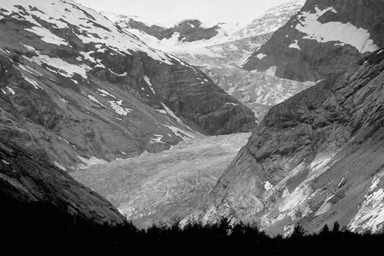
\includegraphics[width=288pt]{../img/02.png}
	\caption{The original image}
\end{figure}

\begin{figure}[H]
	\centering
	% pt = px * 72 / DPI
	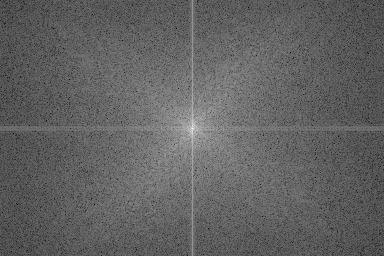
\includegraphics[width=288pt]{../result/dft-spectrum.png}
	\caption{The centered Fourier spectrum}
\end{figure}

\begin{figure}[H]
	\centering
	% pt = px * 72 / DPI
	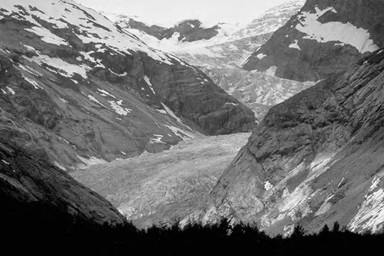
\includegraphics[width=288pt]{../result/dft-double.png}
	\caption{The real part of the IDFT of the DFT}
\end{figure}


% -------------------- Discussion ------------------------
\subsubsection{Analysis}

\paragraph{}


% -------------------- Algorithm ------------------------
\subsubsection{Algorithm}

\begin{algorithm}[H]
\centering
\caption{Histogram Equalization}
  \begin{algorithmic}[1]
    \Function{dft2d}{$input\_img$, flags}
      \State \Return $output\_img$
    \EndFunction
  \end{algorithmic}
\end{algorithm}

% -------------------- Fast Fourier Transform ------------------------

\subsection{Fast Fourier Transform}

% -------------------- Results ------------------------
\subsubsection{Results}
\begin{figure}[H]
	\centering
	% pt = px * 72 / DPI
	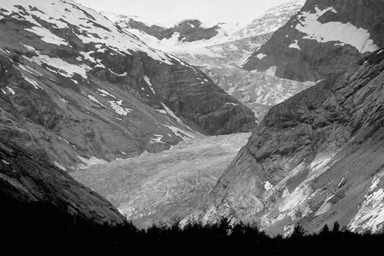
\includegraphics[width=288pt]{../img/02.png}
	\caption{The original image}
\end{figure}

\begin{figure}[H]
	\centering
	% pt = px * 72 / DPI
	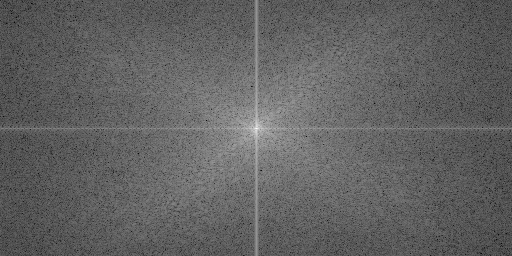
\includegraphics[width=384pt]{../result/fft-spectrum.png}
	\caption{The centered Fourier spectrum}
\end{figure}

\begin{figure}[H]
	\centering
	% pt = px * 72 / DPI
	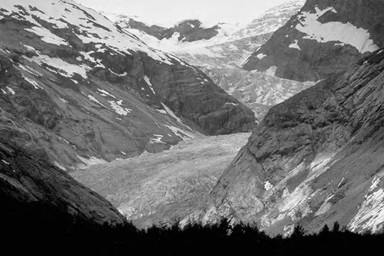
\includegraphics[width=288pt]{../result/fft-double.png}
	\caption{The real part of the IDFT of the DFT}
\end{figure}

% -------------------- Discussion ------------------------
\subsubsection{Analysis}

\paragraph{}


% -------------------- Algorithm ------------------------
\subsubsection{Algorithm}

\begin{algorithm}[H]
\centering
\caption{Histogram Equalization}
  \begin{algorithmic}[1]
    \Function{fft2d}{$input\_img$, flags}
      \State \Return $output\_img$
    \EndFunction
  \end{algorithmic}
\end{algorithm}

% -------------------- Spatial Filtering ------------------------
\subsection{Filtering in the Frequency Domain}

% -------------------- Results ------------------------
\subsubsection{Results}

\begin{figure}[H]
	\centering
	% pt = px * 72 / DPI
	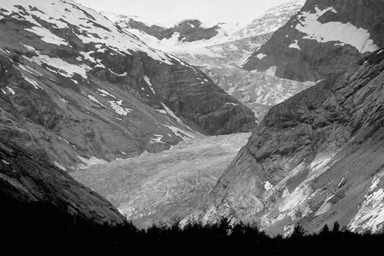
\includegraphics[width=288pt]{../img/02.png}
	\caption{The original image}
\end{figure}

\begin{figure}[H]
	\centering
	% pt = px * 72 / DPI
	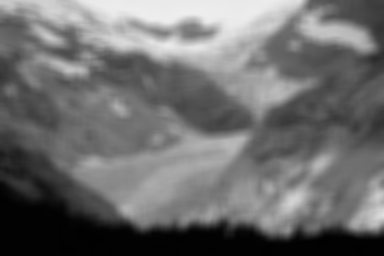
\includegraphics[width=288pt]{../result/average-11-11.png}
	\caption{Smoothed image with $11 \times 11$ averaging filter}
\end{figure}

\begin{figure}[H]
	\centering
	% pt = px * 72 / DPI
	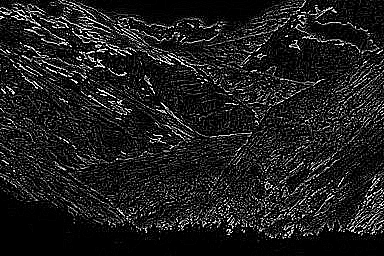
\includegraphics[width=288pt]{../result/laplacian.png}
	\caption{Image filtered with $3 \times 3$ Laplacian filter}
\end{figure}

\begin{figure}[H]
	\centering
		\[ \begin{bmatrix}
			-1 & -1 & -1 \\
			-1 &  8 & -1 \\
			-1 & -1 & -1
		\end{bmatrix} \]
\caption{Laplacian filter}
\end{figure}

\begin{description}
\item[Note] \hfill \\
To obtain a sharpened image with the result of a laplacian filter, we can combine the original image with the filtered result. Because the laplacian filter used here has a positive center, the sharpened image can be produced by:

$$g(x,y) = f(x, y) + laplacian(x, y)$$

where $g(x, y)$, $f(x, y)$, and $laplacian(x, y)$ are intensity values at the pixels of coordinate $(x, y)$ in the sharpened image, original image, and the laplacian filtered image, respectively.
\end{description}


% ---------------------- Discussion ---------------------------
\subsubsection{Discussion}

% ---------------------- Algorithm ---------------------------
\subsubsection{Algorithm}

\begin{description}
\item[Note] \hfill \\
The textbook uses zero padding for the example of correlation, but it also mentions that duplicates or mirror values can be used for padding (see side notes on P169). Here I use the duplicate of the neighborhood center for padding when dealing with borders because it produces a more natural result.

\end{description}

\begin{algorithm}[H]
\centering
\caption{Filter}
  \begin{algorithmic}[1]
    \Function{filter2d\_freq}{$input\_img, filter$}
     \State \Return $output\_img$ 
    \EndFunction
  \end{algorithmic}
\end{algorithm}

\bibliographystyle{acm}

\end{document}